
%% bare_jrnl.tex
%% V1.4
%% 2012/12/27
%% by Michael Shell
%% see http://www.michaelshell.org/
%% for current contact information.

% *** Authors should verify (and, if needed, correct) their LaTeX system  ***
% *** with the testflow diagnostic prior to trusting their LaTeX platform ***
% *** with production work. IEEE's font choices can trigger bugs that do  ***
% *** not appear when using other class files.                            ***
% The testflow support page is at:
% http://www.michaelshell.org/tex/testflow/

%%*************************************************************************
%% Legal Notice:
%% This code is offered as-is without any warranty either expressed or
%% implied; without even the implied warranty of MERCHANTABILITY or
%% FITNESS FOR A PARTICULAR PURPOSE! 
%% User assumes all risk.
%% In no event shall IEEE or any contributor to this code be liable for
%% any damages or losses, including, but not limited to, incidental,
%% consequential, or any other damages, resulting from the use or misuse
%% of any information contained here.
%%
%% All comments are the opinions of their respective authors and are not
%% necessarily endorsed by the IEEE.
%%
%% This work is distributed under the LaTeX Project Public License (LPPL)
%% ( http://www.latex-project.org/ ) version 1.3, and may be freely used,
%% distributed and modified. A copy of the LPPL, version 1.3, is included
%% in the base LaTeX documentation of all distributions of LaTeX released
%% 2003/12/01 or later.
%% Retain all contribution notices and credits.
%% ** Modified files should be clearly indicated as such, including  **
%% ** renaming them and changing author support contact information. **
%%
%% File list of work: IEEEtran.cls, IEEEtran_HOWTO.pdf, bare_adv.tex,
%%                    bare_conf.tex, bare_jrnl.tex, bare_jrnl_compsoc.tex,
%%                    bare_jrnl_transmag.tex
%%*************************************************************************

\documentclass[12pt,draftclsnofoot,onecolumn,journal]{IEEEtran}


% Some very useful LaTeX packages include:
% (uncomment the ones you want to load)

% *** MISC UTILITY PACKAGES ***
%
%\usepackage{ifpdf}
% Heiko Oberdiek's ifpdf.sty is very useful if you need conditional
% compilation based on whether the output is pdf or dvi.
% usage:
% \ifpdf
%   % pdf code
% \else
%   % dvi code
% \fi
% The latest version of ifpdf.sty can be obtained from:
% http://www.ctan.org/tex-archive/macros/latex/contrib/oberdiek/
% Also, note that IEEEtran.cls V1.7 and later provides a builtin
% \ifCLASSINFOpdf conditional that works the same way.
% When switching from latex to pdflatex and vice-versa, the compiler may
% have to be run twice to clear warning/error messages.

% *** CITATION PACKAGES ***
%
%\usepackage{cite}
% cite.sty was written by Donald Arseneau
% V1.6 and later of IEEEtran pre-defines the format of the cite.sty package
% \cite{} output to follow that of IEEE. Loading the cite package will
% result in citation numbers being automatically sorted and properly
% "compressed/ranged". e.g., [1], [9], [2], [7], [5], [6] without using
% cite.sty will become [1], [2], [5]--[7], [9] using cite.sty. cite.sty's
% \cite will automatically add leading space, if needed. Use cite.sty's
% noadjust option (cite.sty V3.8 and later) if you want to turn this off
% such as if a citation ever needs to be enclosed in parenthesis.
% cite.sty is already installed on most LaTeX systems. Be sure and use
% version 4.0 (2003-05-27) and later if using hyperref.sty. cite.sty does
% not currently provide for hyperlinked citations.
% The latest version can be obtained at:
% http://www.ctan.org/tex-archive/macros/latex/contrib/cite/
% The documentation is contained in the cite.sty file itself.


% *** GRAPHICS RELATED PACKAGES ***
%
\ifCLASSINFOpdf
   \usepackage[pdftex]{graphicx}
  % declare the path(s) where your graphic files are
  % \graphicspath{{../pdf/}{../jpeg/}}
  % and their extensions so you won't have to specify these with
  % every instance of \includegraphics
  % \DeclareGraphicsExtensions{.pdf,.jpeg,.png}
\else
  % or other class option (dvipsone, dvipdf, if not using dvips). graphicx
  % will default to the driver specified in the system graphics.cfg if no
  % driver is specified.
  % \usepackage[dvips]{graphicx}
  % declare the path(s) where your graphic files are
  % \graphicspath{{../eps/}}
  % and their extensions so you won't have to specify these with
  % every instance of \includegraphics
  % \DeclareGraphicsExtensions{.eps}
\fi
% graphicx was written by David Carlisle and Sebastian Rahtz. It is
% required if you want graphics, photos, etc. graphicx.sty is already
% installed on most LaTeX systems. The latest version and documentation
% can be obtained at: 
% http://www.ctan.org/tex-archive/macros/latex/required/graphics/
% Another good source of documentation is "Using Imported Graphics in
% LaTeX2e" by Keith Reckdahl which can be found at:
% http://www.ctan.org/tex-archive/info/epslatex/
%
% latex, and pdflatex in dvi mode, support graphics in encapsulated
% postscript (.eps) format. pdflatex in pdf mode supports graphics
% in .pdf, .jpeg, .png and .mps (metapost) formats. Users should ensure
% that all non-photo figures use a vector format (.eps, .pdf, .mps) and
% not a bitmapped formats (.jpeg, .png). IEEE frowns on bitmapped formats
% which can result in "jaggedy"/blurry rendering of lines and letters as
% well as large increases in file sizes.
%
% You can find documentation about the pdfTeX application at:
% http://www.tug.org/applications/pdftex

% *** MATH PACKAGES ***
%
\usepackage[cmex10]{amsmath}
% A popular package from the American Mathematical Society that provides
% many useful and powerful commands for dealing with mathematics. If using
% it, be sure to load this package with the cmex10 option to ensure that
% only type 1 fonts will utilized at all point sizes. Without this option,
% it is possible that some math symbols, particularly those within
% footnotes, will be rendered in bitmap form which will result in a
% document that can not be IEEE Xplore compliant!
%
% Also, note that the amsmath package sets \interdisplaylinepenalty to 10000
% thus preventing page breaks from occurring within multiline equations. Use:
%\interdisplaylinepenalty=2500
% after loading amsmath to restore such page breaks as IEEEtran.cls normally
% does. amsmath.sty is already installed on most LaTeX systems. The latest
% version and documentation can be obtained at:
% http://www.ctan.org/tex-archive/macros/latex/required/amslatex/math/

% *** SPECIALIZED LIST PACKAGES ***
%
%\usepackage{algorithmic}
% algorithmic.sty was written by Peter Williams and Rogerio Brito.
% This package provides an algorithmic environment fo describing algorithms.
% You can use the algorithmic environment in-text or within a figure
% environment to provide for a floating algorithm. Do NOT use the algorithm
% floating environment provided by algorithm.sty (by the same authors) or
% algorithm2e.sty (by Christophe Fiorio) as IEEE does not use dedicated
% algorithm float types and packages that provide these will not provide
% correct IEEE style captions. The latest version and documentation of
% algorithmic.sty can be obtained at:
% http://www.ctan.org/tex-archive/macros/latex/contrib/algorithms/
% There is also a support site at:
% http://algorithms.berlios.de/index.html
% Also of interest may be the (relatively newer and more customizable)
% algorithmicx.sty package by Szasz Janos:
% http://www.ctan.org/tex-archive/macros/latex/contrib/algorithmicx/

% *** ALIGNMENT PACKAGES ***
%
%\usepackage{array}
% Frank Mittelbach's and David Carlisle's array.sty patches and improves
% the standard LaTeX2e array and tabular environments to provide better
% appearance and additional user controls. As the default LaTeX2e table
% generation code is lacking to the point of almost being broken with
% respect to the quality of the end results, all users are strongly
% advised to use an enhanced (at the very least that provided by array.sty)
% set of table tools. array.sty is already installed on most systems. The
% latest version and documentation can be obtained at:
% http://www.ctan.org/tex-archive/macros/latex/required/tools/

% IEEEtran contains the IEEEeqnarray family of commands that can be used to
% generate multiline equations as well as matrices, tables, etc., of high
% quality.

% *** SUBFIGURE PACKAGES ***
%\ifCLASSOPTIONcompsoc
%  \usepackage[caption=false,font=normalsize,labelfont=sf,textfont=sf]{subfig}
%\else
%  \usepackage[caption=false,font=footnotesize]{subfig}
%\fi

\usepackage[caption=false,font=footnotesize]{subfig}
% subfig.sty, written by Steven Douglas Cochran, is the modern replacement
% for subfigure.sty, the latter of which is no longer maintained and is
% incompatible with some LaTeX packages including fixltx2e. However,
% subfig.sty requires and automatically loads Axel Sommerfeldt's caption.sty
% which will override IEEEtran.cls' handling of captions and this will result
% in non-IEEE style figure/table captions. To prevent this problem, be sure
% and invoke subfig.sty's "caption=false" package option (available since
% subfig.sty version 1.3, 2005/06/28) as this is will preserve IEEEtran.cls
% handling of captions.
% Note that the Computer Society format requires a larger sans serif font
% than the serif footnote size font used in traditional IEEE formatting
% and thus the need to invoke different subfig.sty package options depending
% on whether compsoc mode has been enabled.
%
% The latest version and documentation of subfig.sty can be obtained at:
% http://www.ctan.org/tex-archive/macros/latex/contrib/subfig/

% *** FLOAT PACKAGES ***
%
%\usepackage{fixltx2e}
% fixltx2e, the successor to the earlier fix2col.sty, was written by
% Frank Mittelbach and David Carlisle. This package corrects a few problems
% in the LaTeX2e kernel, the most notable of which is that in current
% LaTeX2e releases, the ordering of single and double column floats is not
% guaranteed to be preserved. Thus, an unpatched LaTeX2e can allow a
% single column figure to be placed prior to an earlier double column
% figure. The latest version and documentation can be found at:
% http://www.ctan.org/tex-archive/macros/latex/base/


%\usepackage{stfloats}
% stfloats.sty was written by Sigitas Tolusis. This package gives LaTeX2e
% the ability to do double column floats at the bottom of the page as well
% as the top. (e.g., "\begin{figure*}[!b]" is not normally possible in
% LaTeX2e). It also provides a command:
%\fnbelowfloat
% to enable the placement of footnotes below bottom floats (the standard
% LaTeX2e kernel puts them above bottom floats). This is an invasive package
% which rewrites many portions of the LaTeX2e float routines. It may not workhttps://www.overleaf.com/project/5c170ba37d677a2df920c34a
% with other packages that modify the LaTeX2e float routines. The latest
% version and documentation can be obtained at:
% http://www.ctan.org/tex-archive/macros/latex/contrib/sttools/
% Do not use the stfloats baselinefloat ability as IEEE does not allow
% \baselineskip to stretch. Authors submitting work to the IEEE should note
% that IEEE rarely uses double column equations and that authors should try
% to avoid such use. Do not be tempted to use the cuted.sty or midfloat.sty
% packages (also by Sigitas Tolusis) as IEEE does not format its papers in
% such ways.
% Do not attempt to use stfloats with fixltx2e as they are incompatible.
% Instead, use Morten Hogholm'a dblfloatfix which combines the features
% of both fixltx2e and stfloats:
%
% \usepackage{dblfloatfix}
% The latest version can be found at:
% http://www.ctan.org/tex-archive/macros/latex/contrib/dblfloatfix/

%\ifCLASSOPTIONcaptionsoff
%  \usepackage[nomarkers]{endfloat}
% \let\MYoriglatexcaption\caption
% \renewcommand{\caption}[2][\relax]{\MYoriglatexcaption[#2]{#2}}
%\fi
% endfloat.sty was written by James Darrell McCauley, Jeff Goldberg and 
% Axel Sommerfeldt. This package may be useful when used in conjunction with 
% IEEEtran.cls'  captionsoff option. Some IEEE journals/societies require that
% submissions have lists of figures/tables at the end of the paper and that
% figures/tables without any captions are placed on a page by themselves at
% the end of the document. If needed, the draftcls IEEEtran class option or
% \CLASSINPUTbaselinestretch interface can be used to increase the line
% spacing as well. Be sure and use the nomarkers option of endfloat to
% prevent endfloat from "marking" where the figures would have been placed
% in the text. The two hack lines of code above are a slight modification of
% that suggested by in the endfloat docs (section 8.4.1) to ensure that
% the full captions always appear in the list of figures/tables - even if
% the user used the short optional argument of \caption[]{}.
% IEEE papers do not typically make use of \caption[]'s optional argument,
% so this should not be an issue. A similar trick can be used to disable
% captions of packages such as subfig.sty that lack options to turn off
% the subcaptions:
% For subfig.sty:
% \let\MYorigsubfloat\subfloat
% \renewcommand{\subfloat}[2][\relax]{\MYorigsubfloat[]{#2}}
% However, the above trick will not work if both optional arguments of
% the \subfloat command are used. Furthermore, there needs to be a
% description of each subfigure *somewhere* and endfloat does not add
% subfigure captions to its list of figures. Thus, the best approach is to
% avoid the use of subfigure captions (many IEEE journals avoid them anyway)
% and instead reference/explain all the subfigures within the main caption.
% The latest version of endfloat.sty and its documentation can obtained at:
% http://www.ctan.org/tex-archive/macros/latex/contrib/endfloat/
%
% The IEEEtran \ifCLASSOPTIONcaptionsoff conditional can also be used
% later in the document, say, to conditionally put the References on a 
% page by themselves.

% *** PDF, URL AND HYPERLINK PACKAGES ***
%
%\usepackage{url}
% url.sty was written by Donald Arseneau. It provides better support for
% handling and breaking URLs. url.sty is already installed on most LaTeX
% systems. The latest version and documentation can be obtained at:
% http://www.ctan.org/tex-archive/macros/latex/contrib/url/
% Basically, \url{my_url_here}.


% *** Do not adjust lengths that control margins, column widths, etc. ***
% *** Do not use packages that alter fonts (such as pslatex).         ***
% There should be no need to do such things with IEEEtran.cls V1.6 and later.
% (Unless specifically asked to do so by the journal or conference you plan
% to submit to, of course. )

%%**********************************

% correct bad hyphenation here

\hyphenation{multi-beam}

%%**********************************

\usepackage[mathlines]{lineno}
\renewcommand\linenumberfont{\normalfont\small}
\linenumbers
\begin{document}

%%**********************************

\title{Performance of a double gimbal system for an acoustic sub-bottom probe 
for Mn crust thickness measurements}

%%**********************************

% use \thanks{} to gain access to the first footnote area
% a separate \thanks must be used for each paragraph as LaTeX2e's \thanks
% was not built to handle multiple paragraphs
%

%%**********************************

\author{Mehul Sangekar,~\IEEEmembership{Member,~IEEE,}
        Blair Thornton,~\IEEEmembership{Member,~IEEE,}
        Adrian Bodenmann,        
        and~Tamaki Ura,~\IEEEmembership{Life~Fellow,~IEEE}% <-this % stops a space
\thanks{M. Sangekar is a project researcher with the Institute of Industrial Science, The University of Tokyo (e-mail: mehul@iis.u-tokyo.ac.jp)}
\thanks{B. Thornton is an Associate Professor at the Maritime Robotics Laboratory, Southampton Marine and Maritime Institute, Faculty of Engineering and Physical Science, The University of Southampton, with an adjunct position at the Institute of Industrial Science, The University of Tokyo (e-mail: b.thornton@soton.ac.uk)}
\thanks{A. Bodenmann is a senior research assistant at the Maritime Robotics Laboratory, Southampton Marine and Maritime Institute, University of Southampton, Southampton, UK (e-mail: adrian.bodenmann@soton.ac.uk)}
\thanks{T. Ura is a Distinguished Professor at the Center for Socio-Robotic Synthesis, Kyushu Institute of Technology (e-mail: ura@lsse.kyutech.ac.jp)}
\thanks{This work was supported by the Japanese Ministry of Education under the Program for the "Development of Fundamental Tools for the Utilization of Marine Resources".}}

%%**********************************

% The paper headers
\markboth{IEEE JOURNAL OF OCEANIC ENGINEERING}%
{Shell \MakeLowercase{\textit{et al.}}: Bare Demo of IEEEtran.cls for Journals}

%%**********************************
% make the title area
\maketitle
%%**********************************

\begin{abstract}
This paper evaluates the performance of a double gimbal system for an acoustic sub-bottom probe for measuring crust  thickness in practical Mn crusts surveys. To increase the sampling rate for thickness measurement of Mn crusts obtained by sampling, an acoustic sub bottom probe was made capable of in-situ measurements. However, it was shown in lab experiments that the acoustic reflection intensity of the probe was severely affected by the angle of incidence of the acoustic beam. Since Mn crusts are found abundantly on the slopes of underwater seamounts, a double gimbal system was made to orient the beam parallel to the seafloor using a slope measuring  algorithm. The system has been implemented on the AUV BOSS-A and used for obtaining measurements of Mn crust thickness at No. $5$ Takuyo seamount in Northwest Pacific. The performance of the gimbal system during sea trials is evaluated to demonstrate how it can significantly improve the quality of acoustic reflections obtained from the probe. 
\end{abstract}

\newpage
%%**********************************

\begin{IEEEkeywords}
Acoustic mapping, Sub-bottom, Double gimbal, Mn crusts, Real-time control
\end{IEEEkeywords}

%%**********************************

\IEEEpeerreviewmaketitle

%%**********************************

% 
% form to use if the first word consists of a single letter:
% \IEEEPARstart{A}{demo} file is ....
% 
% form to use if you need the single drop letter followed by
% normal text (unknown if ever used by IEEE):
% \IEEEPARstart{A}{}demo file is ....
% 
% Some journals put the first two words in caps:
% \IEEEPARstart{T}{his demo} file is ....

% An example of a floating figure using the graphicx package.
% Note that \label must occur AFTER (or within) \caption.
% For figures, \caption should occur after the \includegraphics.
% Note that IEEEtran v1.7 and later has special internal code that
% is designed to preserve the operation of \label within \caption
% even when the captionsoff option is in effect. However, because
% of issues like this, it may be the safest practice to put all your
% \label just after \caption rather than within \caption{}.
%
% Reminder: the "draftcls" or "draftclsnofoot", not "draft", class
% option should be used if it is desired that the figures are to be
% displayed while in draft mode.
%
%\begin{figure}[!t]
%\centering
%\includegraphics[width=2.5in]{./images/hires/landselecta.png}
% where an .eps filename suffix will be assumed under latex, 
% and a .pdf suffix will be assumed for pdflatex; or what has been declared
% via \DeclareGraphicsExtensions.
%\caption{Simulation Results.}
%\label{fig_sim}
%\end{figure}

% Note that IEEE typically puts floats only at the top, even when this
% results in a large percentage of a column being occupied by floats.


% An example of a double column floating figure using two subfigures.
% (The subfig.sty package must be loaded for this to work.)
% The subfigure \label commands are set within each subfloat command,
% and the \label for the overall figure must come after \caption.
% \hfil is used as a separator to get equal spacing.
% Watch out that the combined width of all the subfigures on a 
% line do not exceed the text width or a line break will occur.
%
%\begin{figure*}[!t]
%\centering
%\subfloat[Case I]{\includegraphics[width=2.5in]{box}%
%\label{fig_first_case}}
%\hfil
%\subfloat[Case II]{\includegraphics[width=2.5in]{box}%
%\label{fig_second_case}}
%\caption{Simulation results.}
%\label{fig_sim}
%\end{figure*}
%
% Note that often IEEE papers with subfigures do not employ subfigure
% captions (using the optional argument to \subfloat[]), but instead will
% reference/describe all of them (a), (b), etc., within the main caption.


% An example of a floating table. Note that, for IEEE style tables, the 
% \caption command should come BEFORE the table. Table text will default to
% \footnotesize as IEEE normally uses this smaller font for tables.
% The \label must come after \caption as always.
%
%\begin{table}[!t]
%% increase table row spacing, adjust to taste
%\renewcommand{\arraystretch}{1.3}
% if using array.sty, it might be a good idea to tweak the value of
% \extrarowheight as needed to properly center the text within the cells
%\caption{An Example of a Table}
%\label{table_example}
%\centering
%% Some packages, such as MDW tools, offer better commands for making tables
%% than the plain LaTeX2e tabular which is used here.
%\begin{tabular}{|c||c|}
%\hline
%One & Two\\
%\hline
%Three & Four\\
%\hline
%\end{tabular}
%\end{table}

%%**********************Introduction*****************

\section{Introduction}
\label{sec:intro}

Exploration of Manganese crusts (Mn crusts) has gained signifant importance in recent years for their economic and scientific value. 

Mn crusts are found abundantly along the slopes of underwater seamounts. 

For thorough understating of these crusts, estimating their volume and distribution is important.

This  is usually carried out by using camera systems mounted on Remotely Operated Vehicles (ROVs) and sampling using cutting tools mounted on manipulators. 

The spatial resolution obtained from sampling does not provide enough details for volumetric estimation. 

For this, an acoustic sub-bottom probe was developed by our group for in-situ continuous measurements of Mn crusts thickness. 

The acoustic probe focuses a 200 kHz acoustic beam with a diameter of 20 mm at a target 1.5 m away. 

Using the reflected acoustic signal from the surface and the back face of the crust, the thickness of crusts is calculated from the time difference between the two reflections. 

Previous experiments performed by our group in a tank showed that the quality of acoustic reflection is significantly affected by the angle of incidence of the acoustic beam as seen in Figure 1. 

To make practical use of the probe during surveys, an actively controlled double gimbal system was made with a control algorithm which uses the seafloor slope to align the probe parallel to the seafloor. 

The system has been implemented on the survey class Autonomous Underwater Vehicle (AUV) BOSS-A which is a payload oriented vehicle with sensors built specifically for Mn crust surveys. 
It is equipped with the acoustic probe mounted on a double gimbal system as its main payload. 
A high resolution mapping system, capable of centimeter order seafloor reconstructions in color, is implemented on the AUV based on light sectioning. 

These reconstructions can be used to measure accurate slopes of the seafloor. 

However, for actively controlling the gimbals in real-time, a simplified algorithm is made which calculates the plane made by two points on the laser line and range to seafloor measured using the Doppler Velocity Log (DVL). 

The performance of this system during sea trials is elaborated in this paper


Organisation of the paper:

Section 2: Describes the problem with angular reflection 

Section 3: Describes the hardware associated. The acoustic probe, gimbal mechanism, visual mapping system and the control mechanism.

Section 4: Describes the method of analysis of the performance of the system

Section 5: Describes the survey performed in the ocean using this system and analyses the performance of the system.

Section 6: Provides conclusions to the performance of the system.

%%************************Problem****************

%\input{tex/chap2_problem}

%************************Platform*******************************

%\input{tex/chap3_vehicle}

%%***********************Algorithm ***********

%\input{tex/chap4_algo}

%************************Simulation*******************************

%\input{tex/chap5_takuyo}

%%**********************Conclusions******************

\section{Conclusions}

Acoustic probe was developed for continuous measurements of the Mn crust.
Previous results have showed the effect of angle of incidence on the intensity of the acoustic reflection. 
The system was gimbaled to align the probe parallel to the seafloor
AUV was developed using this concept and deployed at an underwater seamount
Results from the trials showed the necessity for such a system to obtain Mn crust thickness measurements.


\section*{Acknowledgements}

The authors thank the crew of R/V Natsushima during the cruises NT15-03, crew of R/V Yokosuka during the cruises YK16-15 and YK17-23, crew of R/V Keirei during the cruise KR16-01 for their help and guidance. We would also like to thank the deployment tem for BOSS-A for their help during the experiments. The project is funded by the Japanese Ministry of Education, Culture, Sports, Science and Technology under the Program for the development of fundamental tools for the utilization of marine resources.

%%*************************************************************************

\bibliographystyle{IEEEtran}
\bibliography{articles}

%%************************IEEEbiography*********************************

\begin{IEEEbiography}[{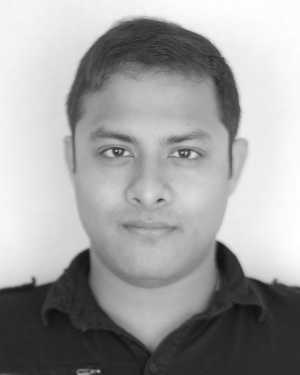
\includegraphics[width=1in,height=1.5in,clip,keepaspectratio]{./images/bio_sange.png}}]{Sangekar Mehul Naresh}
(M’10) received the M.Sc. degree in underwater robotics and Ph.D. degree in ocean technology from The University of Tokyo, Japan, in 2010 and 2014, respectively. He is  working at present as a project researcher at the Thornton Lab, Institute of Industrial Science, The University of Tokyo. Currently, he works on techniques for intelligent, multi-layer resolution mapping of the seafloor using autonomous underwater vehicles. He is also working on developing algorithms for analysis of high resolution seafloor bathymetry and correlating it with other measured seafloor parameters.  
\end{IEEEbiography}

\vskip 0pt plus -1fil

\begin{IEEEbiography}[{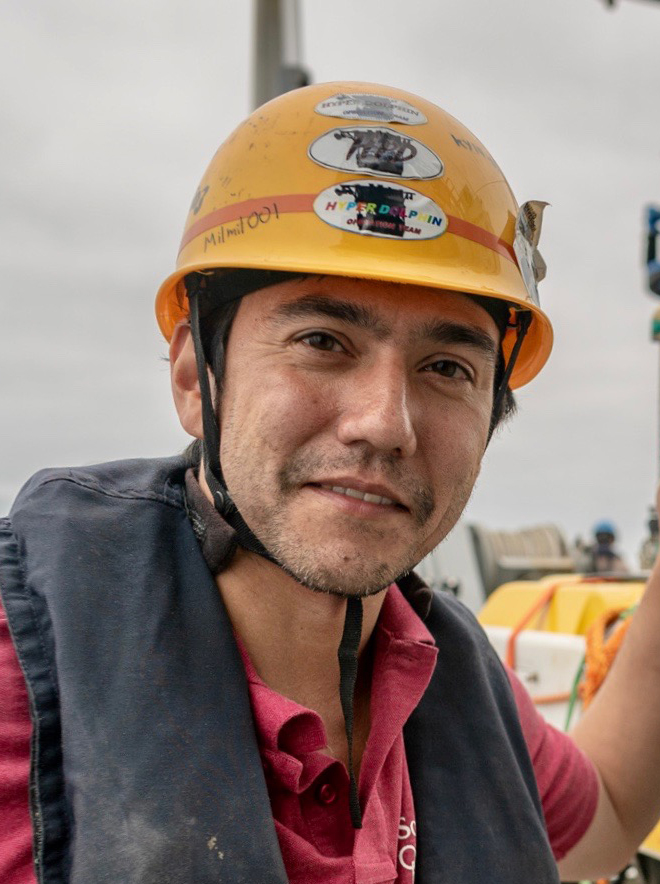
\includegraphics[width=1in,height=1.5in,clip,keepaspectratio]{./images/bio_thorn.jpg}}]{Thornton Blair}
(M’07) received the B.Eng. degree in ship science and the Ph.D. degree in underwater robotics from The University of Southampton, Southampton, U.K., in 2002 and 2006, respectively. He is at present an Associate Professor at the the University of Southampton and also affiliated with the  Ocean Perception Laboratory, Institute of Industrial Science, The University of Tokyo. His research interests involve the development of in-situ sensors and data processing techniques for integrated acoustic, visual, and chemical survey of marine minerals and environment monitoring. He is dedicated to fielding real systems in real environments and overcoming bottlenecks in the flow of information from data collection to human interpretation.
\end{IEEEbiography}

\vskip 0pt plus -1fil

\begin{IEEEbiography}[{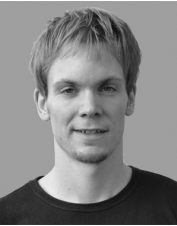
\includegraphics[width=1in,height=1.5in,clip,keepaspectratio]{./images/bio_boden.png}}]{Adrian Bodenmann}
(M’09) received the M.Sc. degree in microengineering from the Ecole Polytechnique Fédérale de Lausanne (EPFL), Lausanne, Switzerland, in 2009. At present he is working at the University of Southampton as a senior research assistant. His research interests are the development of camera systems for high altitude seafloor mapping and algorithms for generating 3D seafloor reconstructions based on photos of the seafloor. He also works on quantifying the certainty in these reconstructions and identifying correlations between identified objects in reconstructions and data from acoustic and chemical sensors.
\end{IEEEbiography}

\vskip 0pt plus -1fil

\begin{IEEEbiography}[{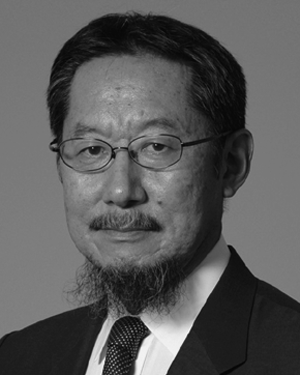
\includegraphics[width=1in,height=1.5in,clip,keepaspectratio]{./images/bio_ura.png}}]{Ura Tamaki}
(M’91–SM’02–F’07) graduated from the Faculty of Engineering, The University of Tokyo, Japan, in 1972 and received the degree of Doctor of Engineering from the same university in 1977. He is at present the Professor emeritus of The University of Tokyo and  Director, Distinguished Professor of Center for Socio-Robotic Synthesis, Kyushu Institute of Technology, and Director of Underwater Technology Center of National Maritime Research Institute. He has developed various types of Autonomous Underwater Vehicles (AUVs) and related application technologies including navigation methods, a new sensing method using a chemical sensor, precise seafloor mapping methods, a precise seabed positioning system with a resolution of a few centimeters, a new sensing system of the thickness of cobalt-rich crust, etc. Finally, he exemplified using these technologies that AUVs are practicable and valuable tools for deep-sea exploration.
\end{IEEEbiography}

\end{document}

%%*************************************************************************